\begin{figure}[H]
\centering
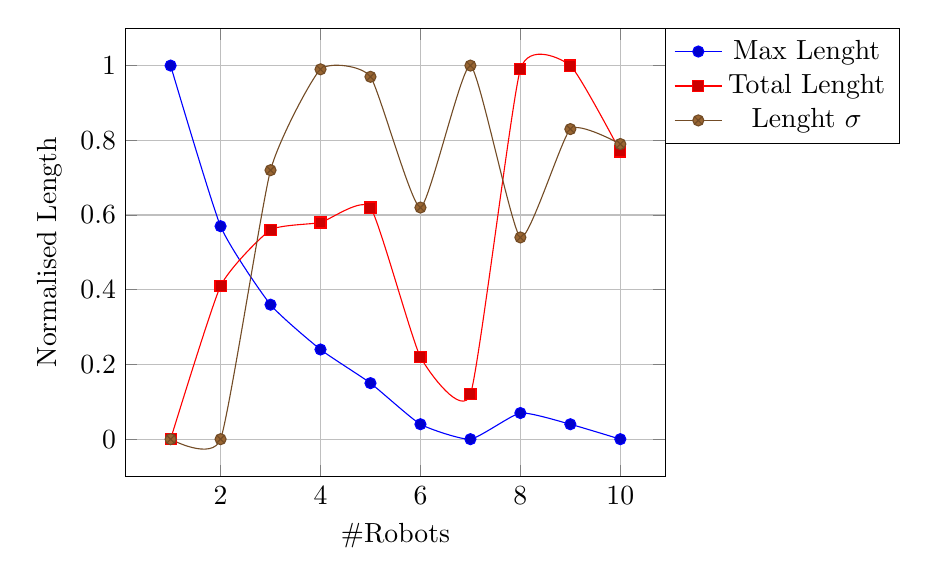
\begin{tikzpicture}
	\begin{axis}[
%		height=9cm,
%		width=9cm,
		grid=major,
                legend style = {at={(1,1)}, anchor=north west},
		xlabel=\#Robots,
		ylabel=Normalised Length,
		smooth,
		tension=0.3
	]

	\addplot coordinates {
(1, 1.00)
(2, 0.57)
(3, 0.36)
(4, 0.24)
(5, 0.15)
(6, 0.04)
(7, 0.00)
(8, 0.07)
(9, 0.04)
(10, 0.00)
	};
	\addlegendentry{Max Lenght}

	\addplot coordinates {
(1, 0.00)
(2, 0.41)
(3, 0.56)
(4, 0.58)
(5, 0.62)
(6, 0.22)
(7, 0.12)
(8, 0.99)
(9, 1.00)
(10, 0.77)
	};
	\addlegendentry{Total Lenght}

	\addplot coordinates {
(1, 0.00)
(2, 0.00)
(3, 0.72)
(4, 0.99)
(5, 0.97)
(6, 0.62)
(7, 1.00)
(8, 0.54)
(9, 0.83)
(10, 0.79)
	};
	\addlegendentry{Lenght $\sigma$}
	\end{axis}
\end{tikzpicture}
\caption{Variation of the performance indexes increasing the number of robots, for the 10x10 grid using the Node Counting algorithm}
\end{figure}